\newtheorem*{Weierstrass}{Weierstrass}
\newtheorem*{existunique}{Existence and Uniqueness}
\chapter{Interpolation and Approximation}
\begin{Weierstrass}
	Suppose $f$ is a continuous real-valued function defined on the real interval $[a,b]$. For every $\epsilon > 0$, there exists a polynomial $p$ such that for all $x$ in $[a,b]$, we have $|f(x)-p(x)| < \epsilon$, or equivalently, the supremum norm $\left\| f-p \right\|< \epsilon$.
\end{Weierstrass}

\section{Interpolation}
Interpolation means we are given a set of data points, usually n+1 data points $(x_i,f(x_i)),i=0,1,...,n$, then to find a polynomial that goes through all of these data points.

\subsection{Basis}
\begin{enumerate}
	\item [I.]
	\textbf{Monomial basis}
	\begin{thm}
		Since the basis $\{1,x,x^2,...,x^n\}$ is complete, any function in the function space can be express using these basis. The interpolating polynomial can be expressed as $P(x) = \sum_{k=0} a_kx^k,\;a_k\in\mathbb{R}$.
	\end{thm}
	
	\begin{ex}
		Find a polynomial interpolation with monomial basis that goes through $(-1,4)$, $(0,3)$ and $(1,6)$.
	\end{ex}
	\begin{solution}
		There are several functions that can go through these three points.
		\[P(x) = 2x^2 + x + 3 \;\; or\;\; P(x) = x^3 + 2x^2 +3\]
		These two all go through the same set of data points.
	\end{solution}

	\item [II.]
	\textbf{Lagrange Interpolation}
	\begin{existunique}
		If $x_i,\; i=0,1,...,n$ are n+1 distinct numbers and f is a function whose values are given at these numbers, then a unique polynomial $P(x)$ with at most degree n exists with
		\[ f(x_k) = P(x_k), \; \forall k=0,1,...,n \]
		
		This polynomial is given by 
		\[ P(x) = \sum_{k=0}^{n} f(x_k)L_{n,k}(x) \]
		where for $k=0,1,2,...,n$,
		\[ L_{n,k} = \underset{i\neq k}{\prod^n_{i=0}} \frac{x-x_i}{x_k-x_i} \]
	\end{existunique}
	
	\begin{ex}
		Find a polynomial interpolation with Lagrange basis that goes through $(-1,4)$, $(0,3)$ and $(1,6)$.
	\end{ex}

	\begin{solution}
		\begin{align*}
		&f(-1)\frac{(x-0)(x-1)}{(-1-0)(-1-1)} +f(0)\frac{(x+1)(x-1)}{(0+1)(0-1)} + f(1)\frac{(x+1)(x-0)}{(1+1)(1-0)} \\
		= & 4\cdot \frac{x(x-1)}{2} + 3\cdot \frac{(x+1)(x-1)}{-1} + 6\cdot \frac{(x+1)x}{2} \\
		= & 2x^2 + x + 3  
		\end{align*}
		
		Recall the existence and uniqueness theorem, the polynomial is unique when its degree is less or euqal to 2 since here we have 3 data point. Compare to the result from previous example 1, we see that the second degree polynomial, $P(x) = 2x^2 + x + 3$, is indeed unique.
	\end{solution}

	\item [III.]
	\textbf{Newton Interpolation}
	\begin{thm}
		Again suppose we have n+1 data points $(x_i,f(x_i),\;i=0,1,...,n$, then Newton basis is defined as 
		\[ N_0(x) = 1,\; N_k(x) = \prod_{j=0}^{k-1} (x-x_j)\,,\;k = 1,2,...,n\]
		And the approximating polynomial can be expressed as:
		\[P(x) = \sum_{k=0}^n f[x_0,x_1,...,x_k] N_k\]
		Where the coefficients, $f[x_0,x_1,...,x_k]$, is the divided difference. Its calculation method is given by the following table.
		\begin{figure} [H]
			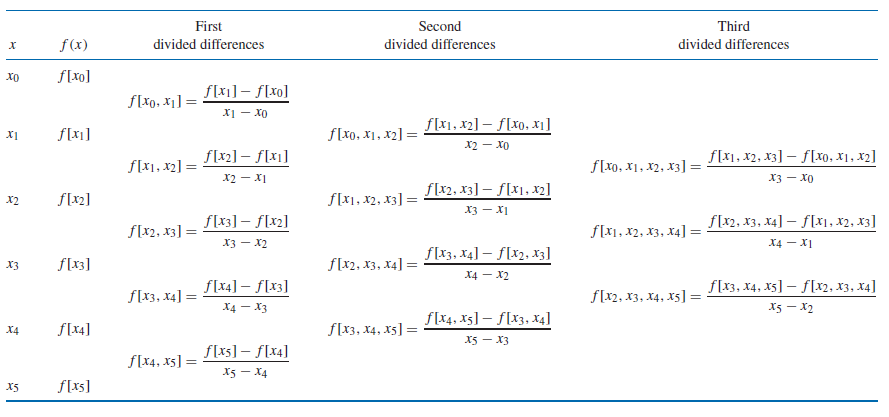
\includegraphics[width=11cm]{img/divided_difference}
			\caption{Divided difference table}
		\end{figure}
	\end{thm}
	
	
	\newpage
	\begin{ex}
		Here is an example
		\begin{figure}[H]
			\centering
			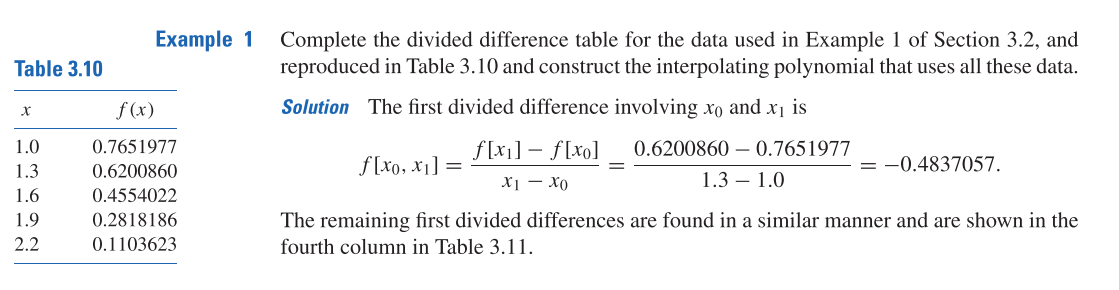
\includegraphics[width=11cm]{img/chapter4_divided_difference_ex.png}
		\end{figure}
		
	\end{ex}
	\begin{solution}
		The solution is 
		\begin{figure}[H]
			\centering
			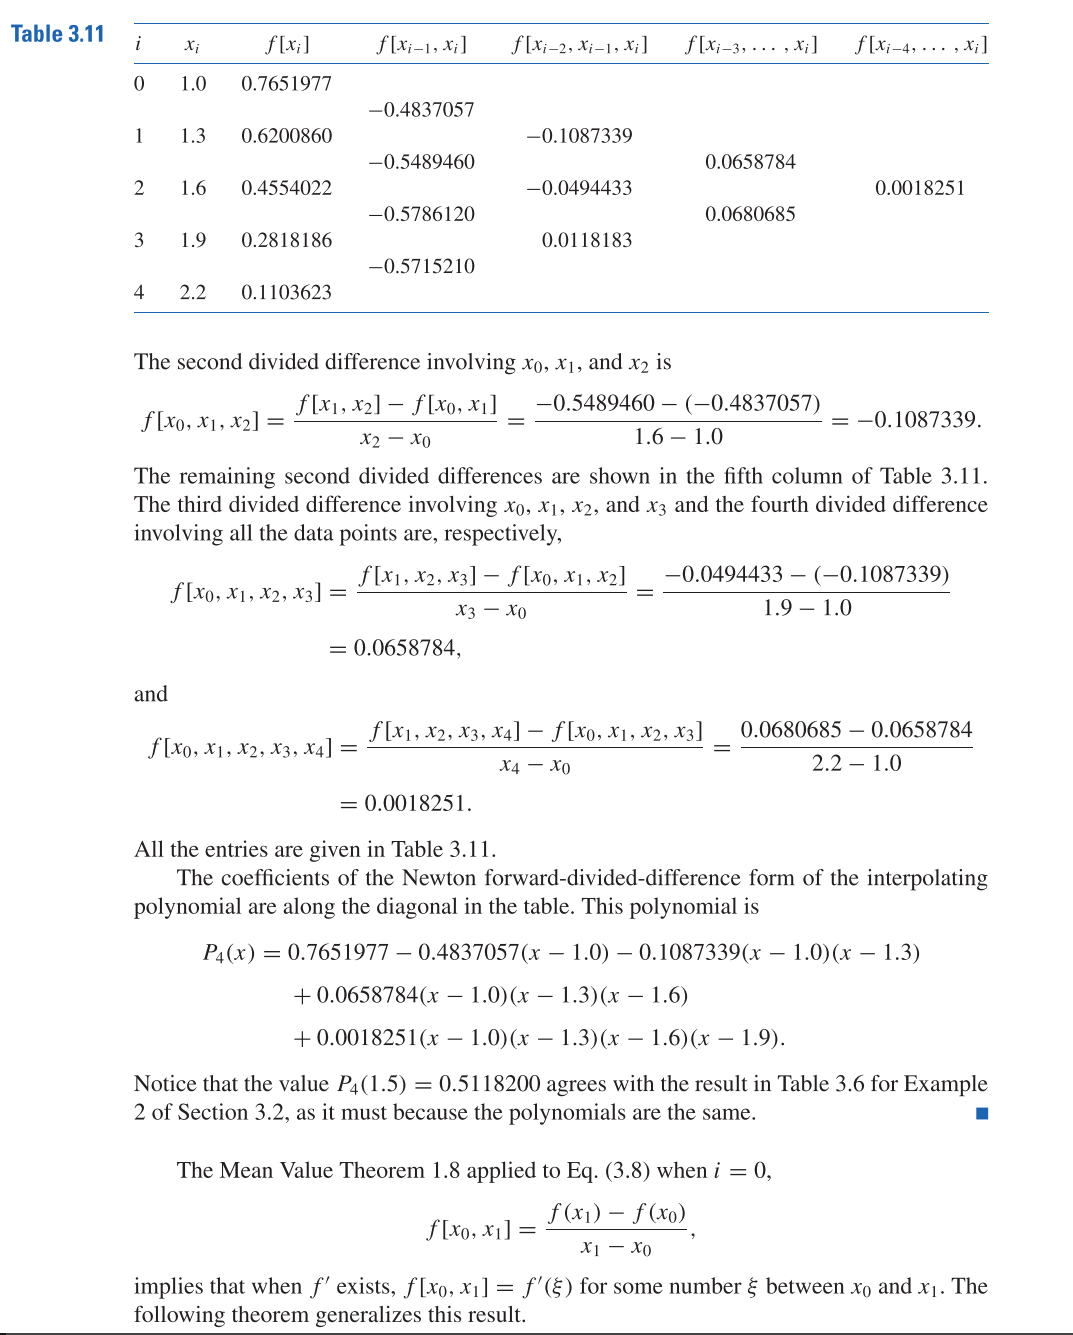
\includegraphics[width=11cm]{img/chapter4_divided_difference_solution.png}
		\end{figure}
	\end{solution}	
	Worth to mention that the cost of computing the Newton form is $O(n^2)$ and evaluating $P(x)$ is $O(n)$ (using nested form), and adding a node $x_{n+1}$ is $O(n)$.
	
	\item [IV.]
	\textbf{Modified Lagrange Interpolation}
	\begin{thm}
		If we have set of n+1 data points $(x_i,f(x_i)),\;i=0,1,...,n$, then the weight is defined as
		\[ \omega_j = \left[ \prod_{\substack{j=0\\k \neq j}}^n (x_j-x_k) \right]^{-1} \]
		and we also define
		\[ L(x) = \prod_{j=0}^n (x-x_j) \]
		Then the approximating polynomial can be expressed as
		\[P(x) = L(x)\sum_{j=0}^n \frac{f(x_j)\omega_j}{x-x_j} \]
	\end{thm}
	\begin{ex}
		Find a polynomial interpolation with barycentric Lagrange basis that goes through $(-1,4)$, $(0,3)$ and $(1,6)$.
	\end{ex}
	\begin{solution}
		First we calculate the weights:
		\begin{align*}
		w_0 &= \frac{1}{(x_0-x_1)(x_0-x_2)} = -\frac{1}{2}\\
		w_1 &= \frac{1}{(x_1-x_0)(x_1-x_2)} = -1 \\
		w_2 &= \frac{1}{(x_2-x_0)(x_2-x_1)} = \frac{1}{2}
		\end{align*}
		
		Now the interpolant is given by
		\begin{align*}
		P(x) &= (x-x_0)(x-x_1)(x-x_2)\left( y_0\frac{w_0}{x-x_0} + y_1\frac{w_1}{x-x_1} +y_2\frac{w_2}{x-x_2} \right) \\
		&= (x+1)x(x-1) \left(\frac{-2}{x+1} + \frac{-3}{x} +\frac{3}{x-1} \right)\\
		\end{align*}
		
		To evaluate the function value at those nodes, we need to do some trick. For example:
		\begin{align*}
		P(0) &= \left. (x+1)x(x-1) \left(\frac{-2}{x+1} + \frac{-3}{x} +\frac{3}{x-1} \right)\right|_{x=0}\\
		&= \left. (x+1)(x-1) \left(\frac{-2x}{x+1} -3 +\frac{3x}{x-1} \right) \right|_{x=0}\\
		&= (0+1)(0-1) \left(0 -3 + 0 \right)\\
		&= 3
		\end{align*}
	\end{solution}
	The efficiency of evaluating weights is $O(n^2)$; computing a function value is $O(n)$; adding an extra node is $O(n)$.
	
	\item [V.] 
	\textbf{The barycentric form} 
	\begin{thm}
		If we have set of n+1 data points $(x_i,f(x_i)),\;i=0,1,...,n$, then the weight is defined as
		\[ \omega_j = \left[ \prod_{\substack{j=0\\k \neq j}}^n (x_j-x_k) \right]^{-1} \]
		Then the approximating polynomial can be expressed as
		\[P(x) = \frac{\sum_{j=0}^n \frac{f(x_j)\omega_j}{x-x_j}}{\sum_{j=0}^n \frac{\omega_j}{x-x_j}} \]
	\end{thm}
	
	
	
	\begin{ex}
		Find a polynomial interpolation with barycentric Lagrange basis that goes through $(-1,4)$, $(0,3)$ and $(1,6)$.
	\end{ex}
	\begin{solution}
		First we calculate the weights:
		\begin{align*}
		w_0 &= \frac{1}{(x_0-x_1)(x_0-x_2)} = -\frac{1}{2}\\
		w_1 &= \frac{1}{(x_1-x_0)(x_1-x_2)} = -1 \\
		w_2 &= \frac{1}{(x_2-x_0)(x_2-x_1)} = \frac{1}{2}
		\end{align*}
		
		Now the interpolant is given by
		\begin{align*}
		P(x) &= \frac{ y_0\frac{w_0}{x-x_0} + y_1\frac{w_1}{x-x_1} +y_2\frac{w_2}{x-x_2} }{ \frac{w_0}{x-x_0} + \frac{w_1}{x-x_1} + \frac{w_2}{x-x_2} } \\
		&= \frac{ \frac{-2}{x+1} + \frac{-3}{x} +\frac{3}{x-1} }{ \frac{-1/2}{x+1} + \frac{-1}{x} + \frac{1/2}{x-1} }
		\end{align*}
		 
		 
		To evaluate the function value at those nodes, we need to do some tricks. For example,
		\[ P(0) = \left. \frac{ x \left(\frac{-2}{x+1} + \frac{-3}{x} +\frac{3}{x-1} \right) }{ x\left(\frac{-1/2}{x+1} + \frac{-1}{x} + \frac{1/2}{x-1}\right)} \right|_{x=0} 
		=\left. \frac{-3 + \frac{-2x}{x+1} +\frac{3x}{x-1}}{-1 + \frac{-x/2}{x+1} + \frac{1/2}{x-1} }\right|_{x=0} = \frac{-3}{-1} = 3 \]
	\end{solution}
	The cost of computing weights $O(n^2)$, evaluating $P(x)$ is $O(n)$, and adding a node is $O(n)$.
\end{enumerate}

\begin{summary}
	Here are the summary of the robustness efficiency of each method:
	\begin{enumerate}
		\item
		Lagrange interpolation: (unstable!)
		\begin{enumerate}
			\item 
			evaluate basis: $O(n^2)$.
			\item 
			evaluate polynomial: $O(n^2)$.
			\item 
			adding an extra node: $O(n^2)$.
		\end{enumerate}
		
		\item 
		Modified Lagrange interpolation (robust)
		\begin{enumerate}
			\item 
			evaluate weights $O(2n^2)$.
			\item 
			evaluate function value: $O(6n)$.
			\item 
			adding an extra node: $O(n)$. 
		\end{enumerate}
		
		\item 
		Barycentric formula: (less robust than MLI)
		\begin{enumerate}
			\item 
			evaluate basis(weights): $O(2n^2)$.
			\item 
			evaluate polynomial: $O(5n)$.
			\item 
			adding an extra node: $O(n)$.
		\end{enumerate}
		\item 
		Newton's divided difference:
		\begin{enumerate}
			\item 
			evaluate coefficients: $O(n^2)$.
			\item 
			evaluate polynomial: $O(n)$.
			\item 
			adding an extra node: $O(n)$.
		\end{enumerate}
		
	\end{enumerate}
\end{summary}

\subsection{Node}
When approximating the known function $f(x)$ or doing interpolation, we can choose a set of points $x_i,\;i=0,1,...,n$, these are the so called nodes. Here is the summary for choosing node:

\begin{enumerate}
	\item 
	Equally spaced nodes on interval $[-1,1]$: 
	
	The barycentric weight in this set of nodes can be written as 
	\[ w_j = (-1)^j \binom{n}{j} = (-1)^j \frac{n!}{j!(n-j)!} \]
	\begin{warning}
		Equally spaced nodes is NOT robust because there is Runge's phenomenon. This phenomenon is not a problem of the barycentric formula but is intrinsic in the underlying interpolation problem. This implies that polynomial interpolation in equally spaced points is highly ill-conditioned: small changes in the data may cause huge changes in the interpolant.
	\end{warning}
	
	\item
	Chebychev nodes of the first kind:
	\[ x_j = \cos\left[ \frac{(2j+1)\pi}{2n+2} \right] ,\;\;j=0,\cdots,n. \]
	
	The barycentric weights of this set of nodes are given by
	\[ w_j = (-1)^j \sin\left[ \frac{(2j+1)\pi}{2n+2}\right] \]
	 
	\item 
	Chebychev nodes of the second kind: 
	\[ x_j = \cos\left(\frac{\pi j}{n}\right), \; j=0,1,...,n.\]
	
	The barycentric weights are given by
	\[ w_j = (-1)^j\delta_j,\;\; \delta_j = \begin{cases}
	1/2,\;\text{$j=0$ or $j=n$}\\
	1,\;\text{otherwise}
	\end{cases} \]
\end{enumerate}

\begin{summary}
	Summing up the key points of nodes:
	\begin{enumerate}
		\item 
		Runge's phenomenon: a small change in data causes a huge change in the interpolant.
		
		\item 
		Equally spaced points are ill-conditioned for interpolation or approximation since Runge's phenomenon happens.
		
		\item 
		Chebychev nodes solve the Runge's phenomenon by clustering points at the boundary.
		
		\item
		Chebychev nodes are obtained by mapping the equally spaced points on a unit semi-circle onto the interval $[-1,1]$.
	\end{enumerate}
	
\end{summary}

\section{Approximation}
Approximation means that we given a known function, and we are going to approximate it. 

\subsection{algorithms}
\begin{enumerate}
	\item [I.]
	Piecewise-Polynomial Approximation.\\
	choose n+1 nodes 
	\[ \{ (x_0, f(x_0)), (x_1, f(x_1)),\cdots, (x_n, f(x_n))\} \]
	then we perform polynomial interpolation.
	\begin{figure} [h]
		\centering
		\includegraphics*[width = 13cm]{img/piecewise_interpolation.png}
	\end{figure}
	\begin{warning}
		The disadvantage of using linear function approximation is that there is likely no differentiability at the nodes, since the approximated function is not smooth.
	\end{warning}
	
	\item [II.]
	Cubic Spline Approximation.\\
	This is the most used piecewise-polynomial interpolation. Here is the procedure of performing a cubic spline approximation:
	\begin{enumerate}
		\item 
		Prepare nodes $\{ (x_0, f(x_0)), (x_1, f(x_1)),\cdots, (x_n, f(x_n))\}$;
		\item
		$S(x)$ is a cubic polynomial, denoted $S_j(x)$, on the subinterval $[x_j, x_{j+1}]$ for each $j = 0, 1,... , n-1$;
		\item 
		$S_j(x_j) = f(x_j)$ and $S_j(x_{j+1}) = f(x_{j+1})$ for each $j = 0, 1,... , n - 1$; 
		\item 
		$S_{j+1}(x_{j+1}) = S_j(x_{j+1})$ for each $j = 0, 1,... , n-2$; (Implied by (b).) 
		\item 
		$S'_{j+1}(x_{j+1}) = S'_j(x_{j+1})$ for each $j = 0, 1,... , n-2$;
		\item 
		$S''_{j+1}(x_{j+1}) = S''_j(x_{j+1})$ for each $j = 0, 1,... , n-2$;
		\item 
		One of the following sets of boundary conditions is satisfied:
		\begin{enumerate}
			\item
			$S''(x_0) = S''(x_n) = 0$ (\textbf{natural boundary} (free boundary));
			\item 
			$S'(x_0) = f'(x_0)$ and $S'(x_n) = f'(x_n)$ (\textbf{clamped boundary}).
		\end{enumerate}
	\end{enumerate} 

	\begin{ex}
		Construct a natural cubic spline that passes through the points $(1, 2)$, $(2, 3)$, and $(3, 5)$.
	\end{ex}
	\begin{solution}
		Since there are 2 subintervals, so there are two cubic functions:
		\begin{align*}
		S_0(x) = a_0 + b_0(x - 1) + c_0(x - 1)^2 + d_0(x - 1)^3,\text{on interval $[1,2]$}\\
		S_1(x) = a_1 + b_1(x - 2) + c_1(x - 2)^2 + d_1(x - 2)^3,\text{on interval $[2,3]$}
		\end{align*}
		On each node, the two cubic functions must satisfy
		\begin{align*}
		2 = &f(1) = a_0\\
		3 = &f(2) = a_0 + b_0 + c_0 + d_0\\
		3 = &f(2) = a_1\\
		5 = &f(3) = a_1 + b_1 + c_1 + d_1
		\end{align*}
		
		Moreover, on each node $S'_0(2) = S'_1(2)$ and $S''_0(2) = S''_1(2)$, these are
		\begin{align*}
		b_0 + 2c_0 + 3d_0 &= b_1\\
		2c_0 + 6d_0 &= 2c_1
		\end{align*} 
		
		Finally, since it requires natural boundary, $S''_0(1) = S''_1(3) = 0$, we have
		\begin{align*}
		2c_0 &= 0\\
		2c_1 + 6d_1 &= 0
		\end{align*}
		
		Solving these 8 equations, we have the 8 parameters, thus
		\[ S(x) = 
		\begin{cases}
		2 + \frac{3}{4}(x-1) + \frac{1}{4}(x-1)^3, \text{for $x\in [1,2]$}\\
		3 + \frac{3}{2}(x-2) + \frac{3}{4}(x-2)^2 - \frac{1}{4}(x-2)^3, \text{for $x\in [2,3]$} 
		\end{cases} \]
	\end{solution}
\end{enumerate}







